%%%%%%%%%%%%%%%%%%%%%%%%%%%%%%%%%%%%%%%%%%%%%%%%%%%%%%%%%%%%%%%%%%%
%                                                                 %
%                            CHAPTER FOUR                         %
%                                                                 %
%%%%%%%%%%%%%%%%%%%%%%%%%%%%%%%%%%%%%%%%%%%%%%%%%%%%%%%%%%%%%%%%%%%

\chapter{VERSIONING GRAPH}\label{ch:graph}

\section{Introduction}

When versioning a data set, researchers very rarely ask whether two objects can be compared.
The data producer often establishes the context in which data objects are sufficiently similar---to use terms from FRBR---\textbf{expressions} of the same \textbf{work}.
Confirming the context prior to making version comparisons is fundamental to ensuring that the resulting versioning graph contains meaningful results.
The data sets described in the following section have sufficient context as established by their producers.
Using the data in these data sets, the model from Chapter \ref{ch:model} is instantiated into versioning graphs.
The graphs are encoded into HTML change logs using RDFa and JSON-LD.
These graphs allow for an analysis of the change between versions, which gives insight into the version identifier.
Finally, a version graph is used to classify the kinds of change separating versions of a data set to determine the utility.

\section{Utilized Data Sets}

\subsection{Noble Gas Data set}

The ``Global Database on \textsuperscript{3}He/\textsuperscript{4}He in on-shore free-circulated subsurface fluids" is a tumultuous database \cite{Polyak2015}.
The first version, published in June 11, 2013, contains 8 files with 194 columns each.
The next version of the database, published March 8, 2015, compiles all the data into a single file and reduces the number of columns to 54, marking a drastic change.
In addition, several columns changed the units with which they reported measurements.
While usage documentation, explaining the content and use of the data, accompanied each version, no records were included indicating what changed between versions.
A change log would be valuable guide with such drastic structural and content changes.
The third and most recent publication came in July 11, 2017, with no changes to the number of files or columns, but many new rows.

\begin{table}
	\caption{Files in the Noble Gas data set.}
	\label{noble_gas_file_table}
	\centering
	\begin{tabular}{|c|c|c|c|c|}
		\hline
		Filename & File Size (Bytes) & Rows & Columns &	Total Cells \\ \hline
		DB\_HE\_6733.xlsx &	2682683 &	6733 &	199 &	1339867 \\
		DB\_final-55-7262\_2015\_03 &	2729060 &	7265 &	54 &	392310 \\
		\_08.xlsx&&&&\\
		NG\_DB\_final\_2017\_07 &	4216595 &	8231 &	54 &	444474 \\
		\_01.xlsx&&&&\\
		\hline
	\end{tabular}
\end{table}

\subsection{Copper Data set}

The Paragenetic Mode for Copper Minerals database became available through collaboration with the author's lab to create new methods of visualizing mineralogy relationships \cite{Morrison2016}.
The first version was collected June 8, 2016, with the update following soon after on August 8, 2016.
Major edits are fairly limited with only 16 column additions and 2 removals between the versions.
Value formats remain consistent from one version to the next, resulting in a much more condensed body of changes, making transitions more easily verifiable.
Compared to the Noble Gas data set, it provides a more stable data platform to implement the versioning model in Chapter \ref{ch:model}.
The data from this work is also more processing friendly, making it agreeable to automatic change log generation.

\begin{table}
	\caption{Files in the Copper data set.}
	\label{copper_file_table}
	\centering
	\begin{tabular}{|c|c|c|c|c|}
		\hline
		Filename & File Size (Bytes) & Rows & Columns &	Total Cells \\ \hline
		ParageneticModeTable\_Cu\_6. &	339175 & 705 &	37 &	26085\\
		8.2016.xlsx&&&&\\
		ParageneticModeTable\_Cu\_8. & 233715 & 685 & 51 & 34935\\
		21.2016.xlsx&&&&\\
		\hline
	\end{tabular}
\end{table}

\section{Implementing the Versioning Model}

The following subsections detail the steps used to implement a versioning graph using the model defined in Chapter \ref{ch:model} and the challenges encountered.
Section \ref{mapping} goes through the decisions made to align the attributes within the Noble Gas dataset and within the Copper data set.
The alignments create a formula to detect changes and assign them to either an \textbf{add}, \textbf{invalidate}, or \textbf{modify} change.
A change log can then use the assignments to organize a presentation of the change data.
The underlying versioning graph exists as linked data encoded within the change log, but can also appear as explicit linked data statements.
The linked data uses a custom-made versioning ontology (VersOn) to express the data model using the \textit{vo:} namespace.
The procedure within this section defines the process used to create versioning graphs found in all the following sections of this chapter.

\subsection{Form a Mapping} \label{mapping}

A mapping specifies the method to determine the \textbf{attributes} of a versioning graph and how to compare them.
For spreadsheets and table-based data, row and column indexes initially seem an ideal attribute, but edits often show the contrary.
The Noble Gas data set needed a mapping to align the spreadsheet's columns since 140 columns were removed from the first version.
The remaining columns in the second version no longer had the same column indexes that they did in version 1 so the column headers were used instead.
The Copper data set retains many of the original columns, but their ordering has changed between versions.
In addition, rows must be aligned since both a row and column attribute are necessary to uniquely identify a cell.
The Noble Gas data set split up its rows across eight files, each file representing a separate region of the Earth.
Instead of forming eight versioning graphs or having eight left-hand versions, the files were collected together into a single abstract collection which is then mapped to the right-hand version.
Creating eight versioning graphs would also form eight separate change logs which doesn't make sense since each file forms only a part of the entire work and the second version collects all entries into a single file.
Multiple left-hand versions also doesn't make sense since this creates one change log and graph, but the files are no longer associated with each other.
Cells need to be uniquely identified since this is where a comparison will be made to determine whether a \textbf{modify} change has occurred in a spreadsheet.

Once aligned, determining which attributes have been added, invalidated, or modified is straight-forward.
Attributes which only exist in the original or left-hand version have been invalidated.
More specifically, a set of attributes \(\mathcal{I} = \mathcal{R}_{l} - \mathcal{R}_{r}\) where \(\mathcal{R}_{l}\) and \(\mathcal{R}_{r}\) correspond to the row identifiers of the left-hand and right-hand versions, respectively.
Likewise, a set of attributes \(\mathcal{A} = \mathcal{R}_{r} - \mathcal{R}_{l}\) contain all the added attributes.
Performing the same operations on the columns result in sets of the added and invalidated columns.
A script then iterates over the remaining cells which exist in both versions to determine if they differ, resulting in a \textbf{modify} change.
The unchanged cells form a set of entries which do not appear in a change log or the versioning graph.
The attributes in these sets are then minted into URIs and linked together into the versioning graph, or they can be used to publish a change log.

\subsection{Generate Versioning Graph}

\begin{figure}
	\centering
	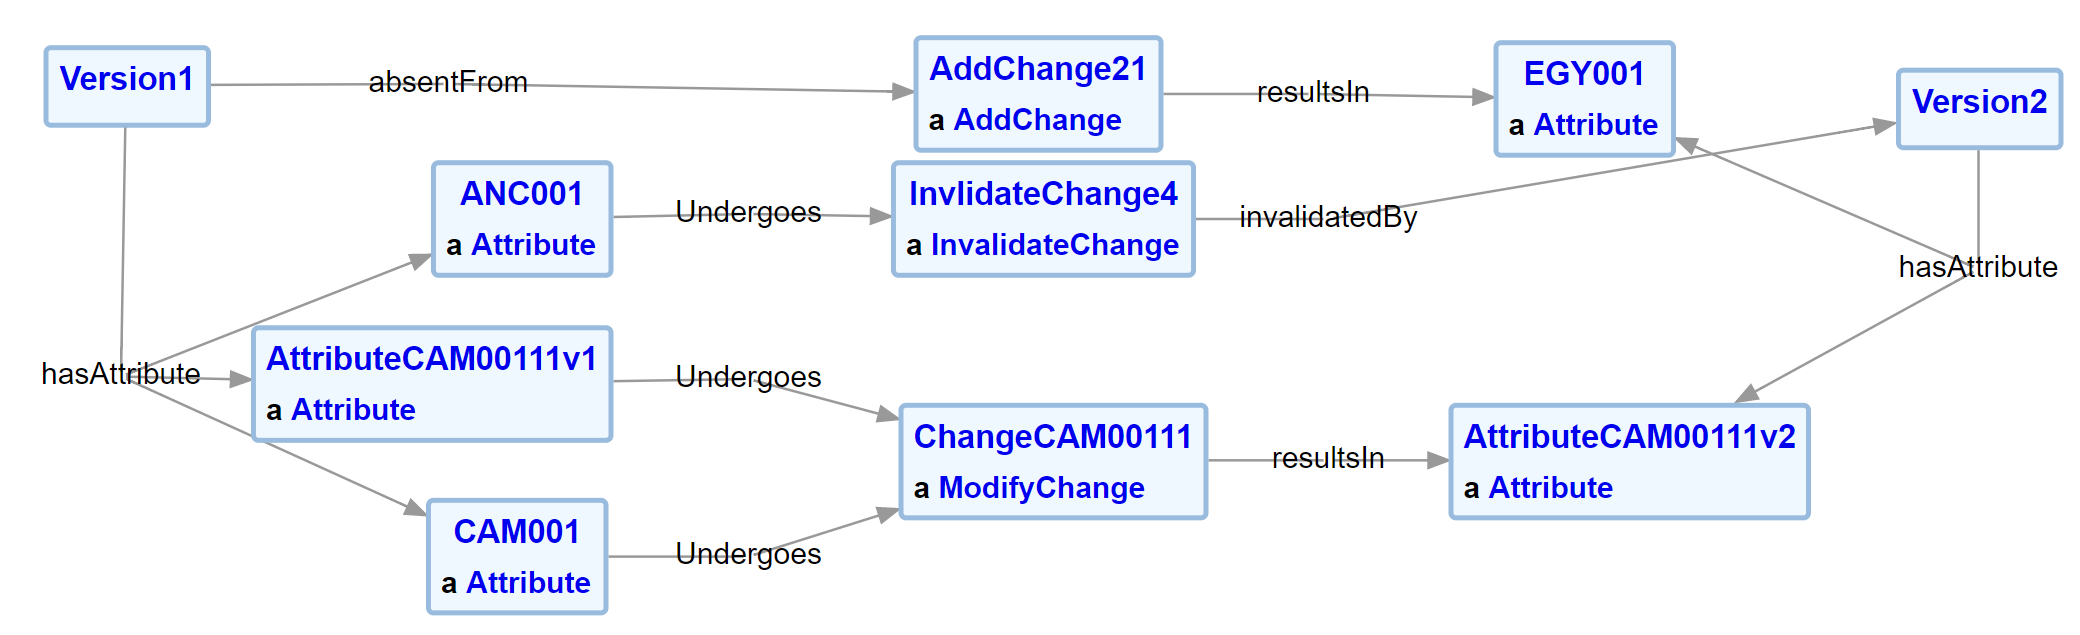
\includegraphics[scale=0.25]{figures/NobleVersion.png}
	\caption{Some initial entries from versions 1 and 2 of the Noble Gas data set}
	\label{NobleGraph1}
\end{figure}
The versioning graphs presented in this section were created by extracting triples from the associated change log which will be covered in Chapter \ref{ch:changelog}.
The statements making up the graph could have alternately been published by writing out the triples directly instead of encoding them into a change log.
Figure \ref{NobleGraph1} displays a subgraph of the Noble Gas data set's versioning graph between versions 1 and 2, highlighting each of the three change operations.
Notice how the versioning graph differs from the provenance graph in Figure \ref{CAM001ProvGraph}.
The versioning graph unpacks the \textit{prov:wasRevisionOf} relationship into explicit components.
These components reveal more detailed differences between version 1 and 2 of CAM001 in the provenance graph which are the differing compilation activities.
\begin{figure}[b]
	\centering
	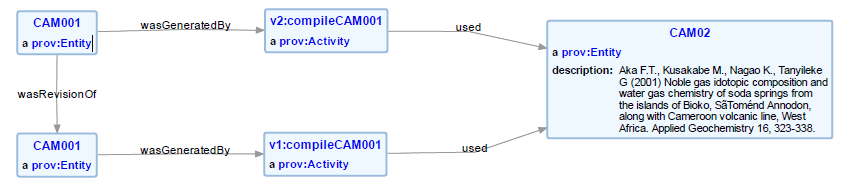
\includegraphics[scale=0.65]{figures/CAM001v1v2.png}
	\caption{Provenance graph for the CAM001 entry of the Noble Gas Database.  Other than the labels, the structure of each data object is very much the same.}
	\label{CAM001ProvGraph}
\end{figure}
The change log encoded the triples in RDFa, resulting in the attribute ``AttributeCAM00111v2" to the right of the \textbf{modify} change.
Because RDFa does not naturally support multiple predicates while also conforming to the content structure of the change log, an attribute was created to combine both the row and column identifier for the changing cell.
Separating the attributes would require multiple dedicated HTML tags which don't appear along with content.
Including these tags would diverge from benefits of encoding triples as attributes.
Figure \ref{NobleGraph1} also shows that even though many columns are added when a new row is added, the row identifier can be used to summarize the columns additions.

Another modification to the implementation differs from the original versioning model.
The \textbf{modify} construction defined in the model only covers the case where a single attribute is sufficient to define a change relation.
The \textbf{modification} captured in spreadsheets describes a cell which requires a row and column identifier to indicate uniquely.
The implementation demonstrates that using multiple attributes is an allowable, sometimes necessary, construction.

Listing \ref{NGA} presents the statements in turtle format necessary to express that the entry EGY001 has been added to the data set from Version 1 to Version 2 as shown along the top of Figure \ref{NobleGraph1}.
The namespace for many of the URIs is \textlangle http://rdfa.info/play/\textrangle.
RDFa allows identifiers to refer to an element on the web page, and the web tool which generated the triples from RDFa, therefore, used its URL as a namespace to produce a valid URI.

\begin{lstlisting}[language=SPARQL, caption=Noble Gas Add in Turtle, label=NGA]
<http://rdfa.info/play/Version1> a vo:Version ;
vo:absentFrom <http://rdfa.info/play/AddChange21> .
<http://rdfa.info/play/AddChange21> a <https://orion.tw.rpi.edu/~blee/VersionOntology.owl#AddChange> ;
vo:resultsIn <http://rdfa.info/play/Attribute21> .
<http://rdfa.info/play/Attribute21> a <https://orion.tw.rpi.edu/~blee/VersionOntology.owl#Attribute> ;
rdfs:label "EGY001"
<http://rdfa.info/play/Version2> a vo:Version ;
vo:hasAttribute <http://rdfa.info/play/Attribute21>
\end{lstlisting}

Figure \ref{CopperGraphVerGraph} shows a similar subgraph from the Copper data set versioning graph.
The graph was assembled using an RDFa change log and also displays a merged attribute on the right side of the \textbf{modify} change.
In the full versioning graph, multiple of each change is present, forming a zipper or ladder-like structure.
As a result, each \textbf{add}, \textbf{invalidate}, or \textbf{modify} change is given separate names for each instantiation.

\begin{figure}
	\centering
	\begin{adjustbox}{addcode={\begin{minipage}{\width}}{
					\caption{Versioning Graph representing the linked data graph with selected entries of additions, invalidations, and modifications. 
			}\end{minipage}},rotate=90,center}
		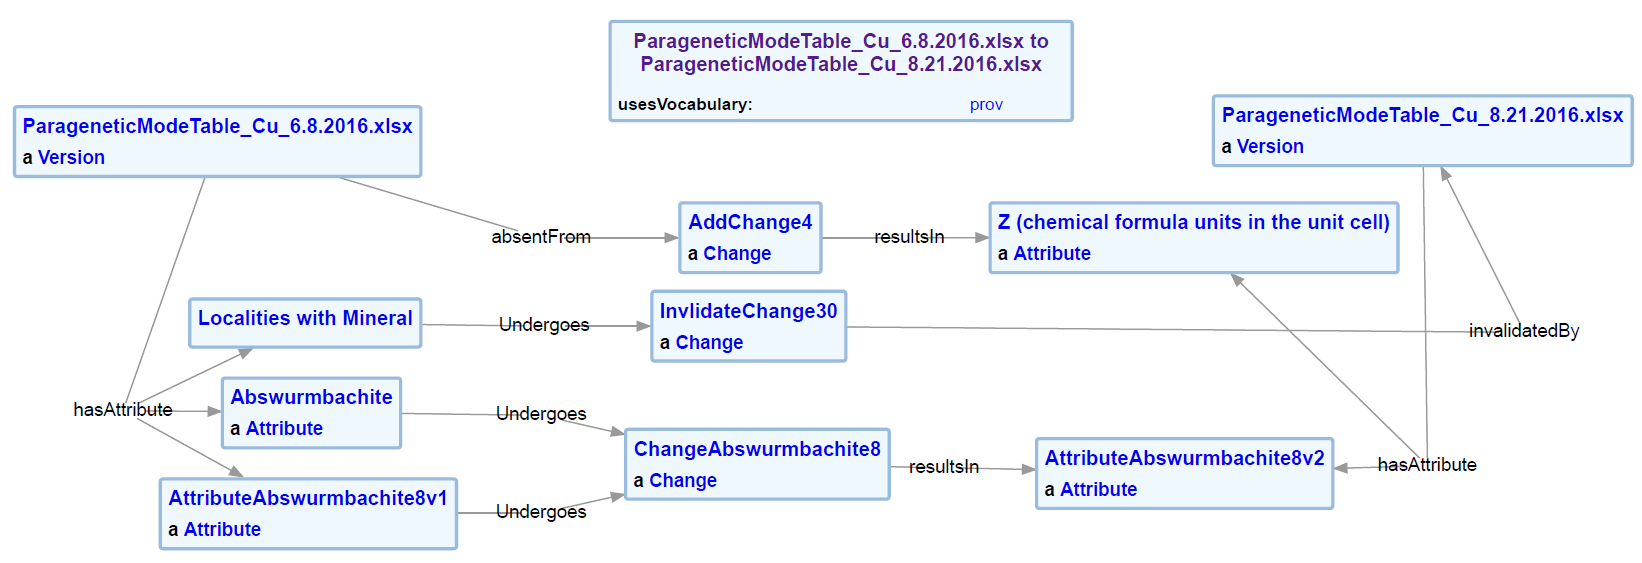
\includegraphics[scale=0.5]{figures/VersioningGraph2.png}%
	\end{adjustbox}
	\label{CopperGraphVerGraph}
\end{figure}

\subsection{Graphs with Multiple Versions}\label{sec:multiver}

Figures \ref{NobleGraph1} and \ref{CopperGraphVerGraph} depict a comparison between only two versions, but a project can contain more than two objects.
Case in point, a third version of the Noble Gas data set was released on July 11, 2017.
Figure \ref{NobleGraph2} shows a subgraph that contains changes from all three versions of the Noble Gas data set.
\begin{figure}
	\centering
	\begin{adjustbox}{addcode={\begin{minipage}{\width}}{
					\caption{Versioning Graph representing the linked data graph with selected entries of additions, invalidations, and modifications after the publication of the third version. 
			}\end{minipage}},rotate=90,center}
		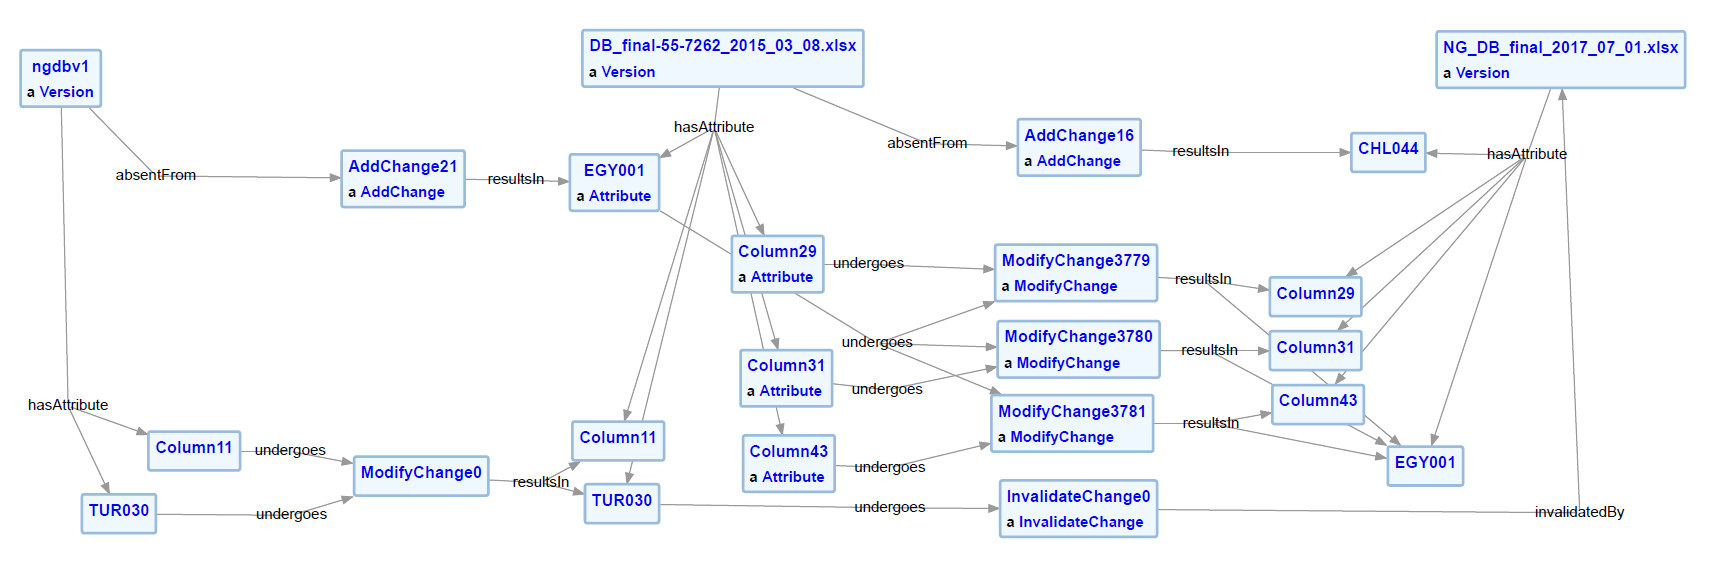
\includegraphics[scale=0.48]{figures/NobleVersion2.png}%
	\end{adjustbox}
	\label{NobleGraph2}
\end{figure}
From the first to second version of the data, EGY001 becomes introduced as an attribute into the data set.
This entry then undergoes a modification change in columns 29, 31, and 43 when comparing versions two and three.
Entry TUR030 goes through a modification change in column 11 from version one to version two.
The entire row, however, becomes invalidated in version three.


Notice the difference in how Figure \ref{NobleGraph1} and Figure \ref{NobleGraph2} refer to columns.
Figure \ref{NobleGraph1} used linked data extracted from a change log employing RDFa, forcing the row identifier and the column identifier into the same concept.
The way nesting works in RDFa means that ChangeCAM00111 cannot back reference multiple concepts in a single statement, therefore AttributeCAM00111v2 was used to imply CAM001.
Figure \ref{NobleGraph2} used linked data extracted from a JSON-LD encoded change log.
Since the log can use explicit statements, the column identifier refers to the entire column and can be used to identify changes in the same column across multiple rows.

\section{Version Graph Analysis}

The versioning graph successfully addresses the concerns of Use Case 1 by capturing all the differences within the Noble Gas data set and within the Copper data set into a versioning graph.
Some additional concerns had to be addressed, such as multiple files in a version and dual attribute identification, during the implementation of the versioning model.
The multiple files in the first version of the Noble Gas data set needed to be collected into a single concept in order to preserve the one-to-one relation between versions.
The grouping simplifies the graph structure as well as reduce the complexity of a change log encoding.

In Chapter \ref{ch:model}, there is only one \textbf{attribute} on each side of the interaction.
Figure \ref{CopperGraphVerGraph}, however, shows two \textbf{attributes} used to characterize the \textit{vo:ModifyChange}.
While the model only shows one \textbf{attribute}, it was found that in some applications, multiple \textbf{attributes} may be necessary to properly model a single change.
The construction does not even need to have the same number \textbf{attributes} on both sides of the \textbf{change}.
The flexibility becomes important when trying to model, for example, a single location entry being split into separate latitude and longitude entries.

The version graph's construction allows multiple versions to be linked together.
The graph provides not only greater continuity than Schema.org's properties, but also greater detail than PROV's versioning properties.
Continuity is important since many versioning linked data alternatives view version change as a single contained \textbf{activity}.
When linking together multiple versions using a versioning graph, the relationship between non-adjacent editions becomes implied in the graph's structure.
The natural pathway between \textbf{attributes} in non-adjacent \textbf{versions} holistically considers the relationships among all \textbf{attributes} along that path.
In comparison, other models only capture activity between the adjacent versions.

The model struggles with discontinuous changes to an \textbf{attribute} across multiple versions.
Since the model does not capture when an \textbf{attribute} doesn't change, it is possible for an \textbf{attribute} in an earlier \textbf{version} to become disconnected from later \textbf{versions} due to inactivity.
For example, in Figure \ref{NobleGraph2}, column 31 of EGY001 becomes modified transitioning into the third version.
If that column underwent no activity in the next transition but changed from version four to five, the connection between all the column 31s would no longer be continuous.
This poses a problem for executing queries in a triple store which rely on graph traversals, but no path exists between disconnected \textbf{attributes}.

\section{Summary}

The results in this chapter implements the versioning model and demonstrates the process and challenges experienced in this endeavor.
The entries in a data set is separated into groups of additions, invalidations, modifications, and unmodified by their attributes.
The grouping occurs over multiple files in the first version of the Noble Gas data set, and the solution was to collect them into a single unit.
The collection keeps the files as one unit, but does not end up addressing other approaches to multi-part versions.

These operational groups organizes the data into a form to publish into a versioning graph.
The approach used to create the graph involves extracting the linked data from a marked up change log.
The decision resulted in constrained representations of the versioning graph, resulting from demands of the encoding methods.
Graphs created using freer form statements, such as the one in Figure \ref{NobleGraph2}, demonstrate an opportunity enable querying over different dimensions of the data.
Changes for specific columns can be queries as easily as individual rows.

The ability to link changes of multiple versions together results as a side effect of the model construction.
Continuously linked changes opens up avenues of exploration to follow change as it propagates through versions.
While change logs will provide a more focused comparison, a triple store with a multi-version graph would give a more global history of the work.
Considering the Noble Gas data set's versioning graph's size, many versions may be difficult to store with large, volatile data sets.

Many statements are necessary to implement a single change in the versioning graph.
The number of statements required may place a limit on how well a version graph can reasonably represent two drastically different versions.
Difficulties with overly large change logs are encountered and discussed further in Chapter \ref{ch:changelog}.
